\documentclass{scrartcl}
\usepackage[a4paper,left=1in,right=1in,top=1.2in,bottom=1in]{geometry}
\usepackage{siunitx}
\usepackage{graphicx}
\usepackage{gensymb}
\setkomafont{disposition}{\normalfont\bfseries}

%title
\title{Exercise 06:\\Tuning curves and receptive fields}
\subtitle{Theoretical Neuroscience I}
\author{Maria del Cerro \and Johannes G\"atjen \and Lorena Morton}

%use these for structure/overview
\newcommand\Question{%
  \textbf{Question:}%
}
\newcommand\Answer{%
  \textbf{Answer:}%
}

\begin{document}
\maketitle

We are provided with two Matlab functions for ``mysterious neurons'' MN1 and MN2, which take an image as an input parameter and return the firing rate of the neuron. We investigate their properties by giving them different images of size $50\times 50$ pixels and observing their responses.

\section{Tuning curve}

First we investigate if the neurons are selective for bars of specific orientations. We use twelve different orientations and repeatedly stimulate the neurons with different inputs to obtain an average response for a specific orientation and the standard deviation of the neuronal responses. This is repeated for both `on bars' and `off bars'. The results are plotted in Figure \ref{tuning}. The neuronal responses are virtually identical between the `on bar' and the `off bar' stimuli. MN1 has a maximum sensitivity to bars with an orientation of 30\degree and MN2 is most sensitive to bars with an orientation of 60\degree. Moreover, MN1 has a much higher standard deviation of the firing rate at its peak sensitivity than MN2 does. This means, that MN1 can have both high and low responses when the bar orientation is `correct', whereas MN2 always has a strong response to bars with the preferred orientation.


\begin{figure}
\centering
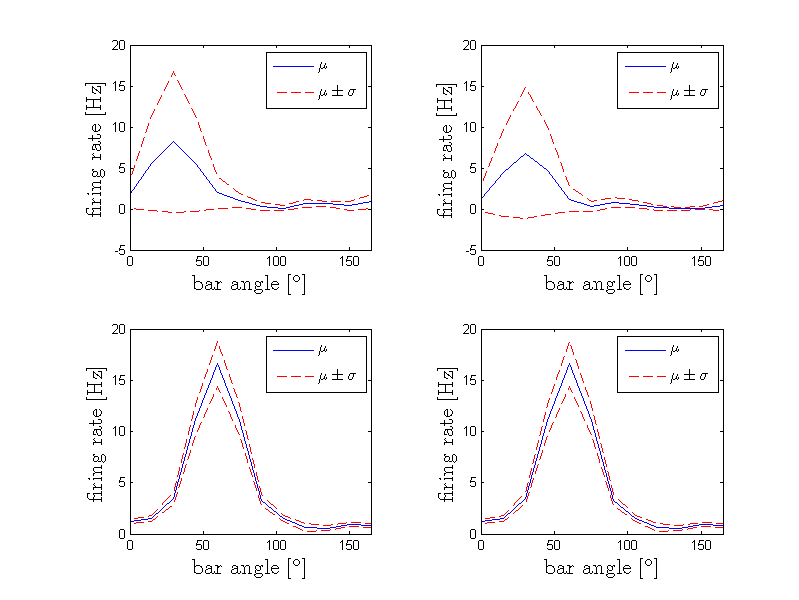
\includegraphics[trim = {1.3cm 0.5cm 1.8cm 0.9cm}, width=\textwidth, clip]{../pics/tuning_on_off}
\caption{The neuron's average firing rate $\mu$ (blue) plus and minus the standard deviation $\sigma$ (dashed red) plotted as a function of the orientation of bars at random positions in the stimulus image. Left column: `On bar'. Right column: `Off bar'. Top row: MN1. Bottom row: MN2. MN1 is most sensitive to bars with an orientation of 30\degree and the standard deviation increases strongly with the neuron's responsiveness. MN2 is most sensitive to bars with an orientation of 60\degree and the standard deviation also increases with a larger response, but to a much lesser extent.}
\label{tuning}
\end{figure}

\section{Response-weighted average stimulus}
We repeatedly stimulate the neurons with random images and compute the response-weighted average stimulus. We do this for `on spot', `off spot' and `white noise' stimuli. The results are shown in Figure \ref{avestim}.

The average stimuli for MN1 show a clear stripe pattern at the angle indicated by the tuning curve. With the `on spot' stimulus we see light stripes on a dark background, with the `off spot' we see dark stripes on a light background and with the `white noise' we see both light and dark stripes on a background of medium intensity. The average stimuli show, that the neuron is not only sensitive to orientations of bars, but also to the position, which explains the high variance in the average response: When a bar is in the correct orientation, but at the wrong position, the neuron's firing rate is decreased instead of increased. We can conclude that MN1 is a simple neuron.

The average stimuli for MN2 only show the extent of the receptive field and that it is more sensitive to stimuli at the center of the receptive field. This indicates, that the neuron has no preference for the positions of bar stimuli, although we have shown with the tuning curve, that it is sensitive to the orientation. This also explains the comparatively low standard deviation of the neuron's firing rate. Because the position is irrelevant to the neuron \textit{all} bars with the correct orientation will elicit a high response. In conclusion, MN2 is a complex neuron.

The `on spot' and `off spot' stimuli require fewer trials than `white noise' to obtain a weighted average stimulus, with which you can see the structure of the preferred stimulus. However, there is no distinction between areas of the image that the neuron does not care about and areas that are sensitive to the same stimulus intensity as the majority of the example stimulus. Only by looking at the preferred stimulus obtained from both stimulus types can we conclude, that the receptive field of the neuron does not extend all the way to the edge of the input images, and that it is more sensitive to stimuli in the center of the receptive field. By using the `white noise' stimulus on the other hand, we see both the regions that are sensitive to light and dark stimuli, and can simultaneously differentiate them from regions the neuron is indifferent to. However, we do not see a clear difference areas outside of the receptive field and areas of the receptive field that are ignored.

\begin{figure}
\centering
\frame{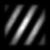
\includegraphics[width=0.3\textwidth]{../pics/ave_on1}} \hspace{3pt}
\frame{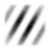
\includegraphics[width=0.3\textwidth]{../pics/ave_off1}} \hspace{3pt}
\frame{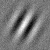
\includegraphics[width=0.3\textwidth]{../pics/ave_wn1}}\\
\vspace{6pt}
\frame{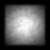
\includegraphics[width=0.3\textwidth]{../pics/ave_on2}} \hspace{3pt}
\frame{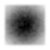
\includegraphics[width=0.3\textwidth]{../pics/ave_off2}} \hspace{3pt}
\frame{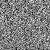
\includegraphics[width=0.3\textwidth]{../pics/ave_wn2}}
\caption{The response-weighted average stimulus images for the mysterious neurons with different stimulus types. Top row: MN1. Bottom row: MN2. Columns left to right: `On spot', `off spot', `white noise'.}
\label{avestim}
\end{figure}

\section{Response-weighted average covariance}

Since MN2 is a complex neuron, calculating the response-weighted average stimulus does not inform us about the neuron's preferred stimuli. We can however calculate the response-weighted average covariance and calculate the principal eigenvectors of the covariance matrix (see Figure \ref{eigen}). This is essentially doing a principal component analysis. The principal eigenvectors of the covariance matrix are those, whose multiples added to the average stimulus elicit the greatest variability in neuronal response. In other words, they are the type of stimulus the neuron ``cares about''.

\begin{figure}
\centering
\begin{tabular}{c c c}
\frame{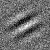
\includegraphics[width=0.3\textwidth]{../pics/eigenvec1_wn}}&
\frame{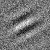
\includegraphics[width=0.3\textwidth]{../pics/eigenvec2_wn}} & \begin{tabular}[b]{c c}
  \frame{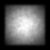
\includegraphics[width=0.145\textwidth]{../pics/eigenvec1_on}}& 
  \frame{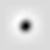
\includegraphics[width=0.145\textwidth]{../pics/eigenvec2_on}} \\
  \frame{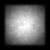
\includegraphics[width=0.145\textwidth]{../pics/eigenvec1_off}} &
  \frame{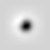
\includegraphics[width=0.145\textwidth]{../pics/eigenvec2_off}}
 \end{tabular}
\end{tabular}
\caption{The eigenvectors of the response-weighted average covariance for MN2 with different stimulus types. Left and center: Eigenvectors of the first and second eigenvalues of the average covariance matrix for `white noise' stimulus. Right: First two eigenvectors for `on spot' and `off spot' (first eigenvector left, `on spot' top). The method works for `white noise' stimuli, but fails for the `spot' stimuli. From the eigenvectors obtained with the `white noise' stimuli we can determine the preferred orientation and spatial frequency for the neuron.}
\label{eigen}
\end{figure}


%include picture
%\begin{figure}
%\centering
%\includegraphics[trim = {1.3cm 0 2cm 0.9cm}, width=\textwidth, clip]{../pics/picname}
%\caption{caption text}
%\label{label}
%\end{figure}
\end{document}